
% < 1 Big Data in der Praxis - Lösungen mit Hadoop, Spark, HBase und Hive. Daten speichern, aufbereiten, visualisieren. 2. erweiterte Auflage, von  Jonas Freiknecht, Stefan Papp, 2018, S
% < 1 https://www.omega.com/en-us/resources/data-loggers
% 0 https://www.researchgate.net/profile/Anne-Ojala/publication/254255682_Eddy_Covariance_A_Practical_Guide_to_Measurement_and_Data_Analysis/links/00b7d51fbaa83999a4000000/Eddy-Covariance-A-Practical-Guide-to-Measurement-and-Data-Analysis.pdf#page=80
Data Logging kann dazu verwendet werden, Code zu debuggen oder große Datenmengen zu speichern, um diese später auszuwerten. Ein Datenlogger ist im Allgemeinen ein Instrument, welches Veränderungen unter bestimmten Bedingungen während einer gewissen Zeitspanne aufzeichnet. Ein Datenlogger verwendet meist Sensoren, um Daten zu sammeln. Anschließend können die Daten ausgelesen, visuell dargestellt und/oder ausgewertet werden. Die Daten, welche von Datenloggern ausglesen werden, betragen meist, Druck, Temperatur, Luftfeuchtigkeit, Spannung oder Stromstärke. \cite{DataLogging} 

Die gespeicherten (geloggten) Daten können dazu verwendet werden, 

\begin{compactitem}
    \item um die Temperatur und die Luftfeuchtigkeit in einem Gebäude zu überprüfen.
    \item Information zur Gebäudewartung zur Verfügung zu stellen, dies betrifft das Heizen, die Belüftung, die Klimatisierung. Diese ständige Überprüfung der Daten kann den Energieverbrauch reduzieren.
    \item die Wachs-Bedingungen von Pflanzen in der Landwirtschaft zu überwachen. 
    \item die Impfstoff-Lagerung in medizinischen Einrichtungen zu überwachen. 
    \item die Temperatur von Lebensmittel zu überprüfen.
\end{compactitem}
\cite{DataLogging}

Logging bieten eine große Flexibilität und eignet sich sehr gut um große Datenmengen zu erfassen und auszuwerten. \cite{BigDataBuch}

\subsection{Herkunft der Daten (Datenpunkte)}
Um die Daten zu loggen, also abzuspeichern, werden diese aus sogenannten Datenpunkten ausgelesen. Diese werden angesprochen und aus ihnen kann dann der aktuelle Wert des Datenpunkts ausgelesen werden.
Datenpunkte welche abgehört werden sind: 

\begin{compactitem}
    \item Daten der Photovoltaik-Anlage am Dach der Firma
    \item die Temperatur in den Firmengebäuden
    \item Kompressor-Druck von Maschinen der Firma
    \item weitere Maschinendaten der Firma (REAL1, REAL178, ...)
\end{compactitem}

\subsection{Log4J}
% < 1 https://books.google.at/books?hl=de&lr=&id=hZBimlxiyAcC&oi=fnd&pg=PA9&dq=log4j&ots=QiOna081Z6&sig=9h3lwPqN-rm07kAHln-tLSUfgJY&redir_esc=y#v=onepage&q=log4j&f=false The Complete Log4j Manual, von: Ceki Gülcü S15
% < 1 https://logging.apache.org/log4j/2.x/
Framework, um Anwendungsmeldungen von JAVA zu loggen.
Das Design von Log4J konzentriert sich vor allem darauf, schnell, flexibel und leicht verständlich zu sein. Da Logging eine Applikation verlangsamen kann, wird vor allem auf die Schnelligkeit Wert gelegt.  \cite{log4JBuch} 

Sehr populär als Logging Package für Java. Logging liefert sehr präzise Informationen über den Ablauf einer Applikation. \cite{log4J}



Anwendungen, welche Log4j verwenden, fordern vom LogManager einen Logger mit einem bestimmten Namen an. Der LogManager sucht den entsprechenden LoggerContext und ruft dann den Logger von diesem ab. 
Wenn der Logger erstellt werden muss, wird er mit der LoggerConfig verknüpft, die entweder a) den gleichen Namen wie der Logger, b) den Namen eines übergeordneten Pakets oder c) die Stamm-LoggerConfig enthält. LoggerConfig-Objekte werden aus Logger-Deklarationen in der Konfiguration erstellt. Die LoggerConfig ist mit den Appendern verbunden, die die LogEvents tatsächlich liefern. \ref{fig:impl:log4jArchitektur} \cite{log4J}

\begin{figure}[h t]
    \centering
    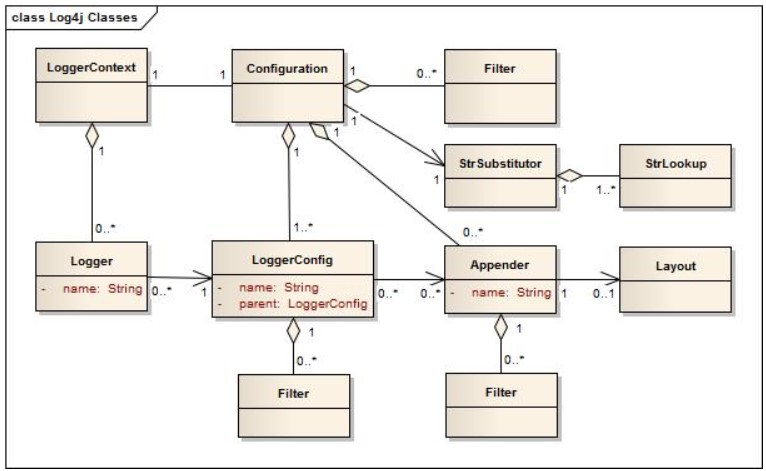
\includegraphics[scale=0.7]{pics/log4jArchitektur.jpg}
    \caption{log4J Architektur \cite{log4J}}
    \label{fig:impl:log4jArchitektur}
\end{figure}